% Hashgrid bilinear-lookup illustration: two cells (blue coarse, green fine),
% with the fragment sample at the same relative position it had inside the
% corresponding cell in scene_intersect.tex.
%
% Relative positions of x_i within each cell (from scene_intersect.tex):
%   blue cell  (bottom-right of 2x2, x∈[3,6], y∈[0,3]):
%        ((3.4-3)/3, (2.55-0)/3) = (0.133, 0.850)
%   green cell (middle of 3x3, x∈[2,4], y∈[2,4]):
%        ((3.4-2)/2, (2.55-2)/2) = (0.700, 0.275)
\documentclass[tikz,border=4pt]{standalone}
\usepackage{tikz}
\usepackage{amsmath}
\usepackage{amssymb}
\usepackage{xcolor}
\usetikzlibrary{positioning, calc, arrows.meta}

\begin{document}
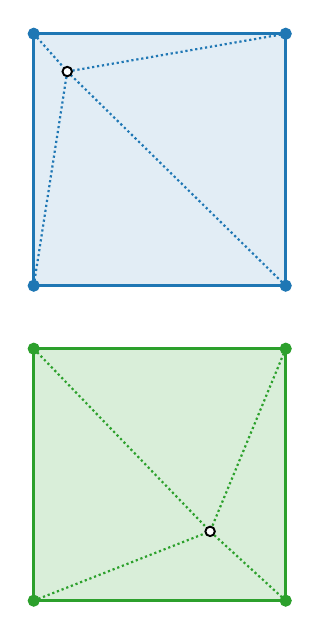
\begin{tikzpicture}[
  font=\sffamily\footnotesize,
]
\definecolor{cgridA}{HTML}{1F77B4}   % blue (coarse)
\definecolor{cgridB}{HTML}{2CA02C}   % green (fine)

% -------- common cell geometry --------
\pgfmathsetmacro{\sz}{3.2}            % side length of each cell in cm

% =====================================================================
% Blue (coarse) cell — on top
% =====================================================================
\begin{scope}[shift={(0,4.0)}]
  % cell
  \fill[cgridA, opacity=0.13] (0,0) rectangle (\sz,\sz);
  \draw[cgridA, line width=1.1pt] (0,0) rectangle (\sz,\sz);

  % sample point at relative (0.133, 0.850)
  \pgfmathsetmacro{\sx}{0.133*\sz}
  \pgfmathsetmacro{\sy}{0.850*\sz}
  \coordinate (sB) at (\sx,\sy);

  % dotted bilinear lines from each corner to the sample
  \draw[cgridA, densely dotted, line width=0.8pt] (0,0)    -- (sB);
  \draw[cgridA, densely dotted, line width=0.8pt] (\sz,0)  -- (sB);
  \draw[cgridA, densely dotted, line width=0.8pt] (0,\sz)  -- (sB);
  \draw[cgridA, densely dotted, line width=0.8pt] (\sz,\sz)-- (sB);

  % corner feature markers
  \foreach \p in {(0,0),(\sz,0),(0,\sz),(\sz,\sz)} {
    \filldraw[cgridA] \p circle (0.07);
  }

  % sample point
  \draw[black, line width=0.7pt, fill=white] (sB) circle (0.06);
\end{scope}

% =====================================================================
% Green (fine) cell — below
% =====================================================================
\begin{scope}[shift={(0,0)}]
  \fill[cgridB, opacity=0.18] (0,0) rectangle (\sz,\sz);
  \draw[cgridB, line width=1.1pt] (0,0) rectangle (\sz,\sz);

  \pgfmathsetmacro{\sx}{0.700*\sz}
  \pgfmathsetmacro{\sy}{0.275*\sz}
  \coordinate (sG) at (\sx,\sy);

  \draw[cgridB, densely dotted, line width=0.8pt] (0,0)    -- (sG);
  \draw[cgridB, densely dotted, line width=0.8pt] (\sz,0)  -- (sG);
  \draw[cgridB, densely dotted, line width=0.8pt] (0,\sz)  -- (sG);
  \draw[cgridB, densely dotted, line width=0.8pt] (\sz,\sz)-- (sG);

  \foreach \p in {(0,0),(\sz,0),(0,\sz),(\sz,\sz)} {
    \filldraw[cgridB] \p circle (0.07);
  }

  \draw[black, line width=0.7pt, fill=white] (sG) circle (0.06);
\end{scope}

\end{tikzpicture}
\end{document}
